% IPCCC 2026 — 5D H-NGAC manuscript
% Numbers: docs/canonical-context.md wins.
% Build: pdflatex main && bibtex main && pdflatex main && pdflatex main
\documentclass[conference]{IEEEtran}
\usepackage{amsmath,amssymb}
\usepackage{booktabs}
\usepackage{graphicx}
\usepackage{url}
\graphicspath{{figures/}}

\begin{document}

\title{Security Dimensionality at Zero Time Cost: A Provenance-Aware 5D H-NGAC Authorization Primitive on FPGA}

\author{
\IEEEauthorblockN{Hassan Karim\IEEEauthorrefmark{1},
Omar Faruque\IEEEauthorrefmark{2},
Abdel-Hameed A.\ Badawy\IEEEauthorrefmark{2},
Sai Sitharaman\IEEEauthorrefmark{3},
Deepti Gupta\IEEEauthorrefmark{4}}
\IEEEauthorblockA{\IEEEauthorrefmark{1}Stable Cyber LLC \quad
\IEEEauthorrefmark{2}Florida International University \quad
\IEEEauthorrefmark{3}Zetafence, Inc. \quad
\IEEEauthorrefmark{4}Texas A\&M University - Central Texas}
}

\maketitle

\begin{abstract}
Real-time robotic and drone system designers often leave authorization out of the control path because software policy engines do not offer decisions within a fixed cycle budget. Operating system scheduling, not policy evaluation, creates non-deterministic latency, so a faster software-based engine does not offer the guarantees required by hard real-time applications. The gap leaves attack classes open that identity-based authorization cannot see, including unsafe-state operation and command injection from compromised but credentialed nodes. State of the art H-NGAC compiles NGAC policy graphs into fixed-width hardware bitmasks so that an authorization decision reduces to a chain of bitwise AND operations. In this paper we extend H-NGAC with two further dimensions, runtime system state and command provenance. We also synthesize these four- and five-dimensional kernels to a Zynq-7020 FPGA. We evaluate the synthesized kernels against six software baselines, and the five-dimensional policy in an adversarial Robot Operating System 2 (ROS~2) scenario against a compromised node that has already authenticated. We found that the added security dimension is free in time. Both kernels resolve in an identical number of clock cycles at every policy size tested, with a closed-form worst case and zero jitter by construction. In software, the same added dimension makes every policy rule 19\% more expensive. Thus, the authorization worst case becomes a synthesis parameter rather than a measurement, and we quantify what that determinism costs in area and in average-case speed.
\end{abstract}

\begin{IEEEkeywords}
access control, NGAC, FPGA, high-level synthesis, real-time systems, robotics, ROS 2, worst-case execution time, provenance, cyber-physical security
\end{IEEEkeywords}

\section{Introduction}

A quadruped inspection robot in maintenance mode should not move. Consider Layla, a field technician replacing a battery pack on a 45~kg platform when a velocity command arrives from a remote operator console. The DDS transport authenticates the console's certificate and delivers the command in well under a millisecond. No layer of that stack asks whether a remote operator is entitled to command motion while a technician holds the interlock. If the platform acts, Layla absorbs the consequence. This failure mode is not hypothetical. CVE-2022-33323 documents unauthorized command execution against Mitsubishi MELFA industrial robots \cite{cve202233323}, and CVE-2021-38425 documents message injection against eProsima Fast DDS, the default ROS~2 transport \cite{cve202138425}.

Robotics platforms leave authorization out of the control path for a defensible reason. Although modern policy engines evaluate rich attribute-based policy, they cannot bound the decision. That is, the latency tail of a software policy decision point is governed by operating system scheduling, preemption and cache state, not by policy evaluation, so a faster engine does not tighten the bound. In our own published measurements, an OPA edge deployment took 1 to 5~ms per decision and an XACML decision point near 50~ms, while a software authorization path averaging 1.14~$\mu$s still produced a single 157~$\mu$s scheduling outlier \cite{karim2026dcas}. A further evaluation, now under review, measured OPA at a 271.491~$\mu$s mean with 13 missed real-time deadlines \cite{karim2026tsngac}. A control loop cannot budget for a tail it cannot bound. Thus engineers place authorization at the perimeter and leave the control path open.

Our research line approaches this as a compilation problem. The hypergraph privilege analysis of Sitharaman et al.\ established that large privilege structures compile into forms that answer set-level questions quickly \cite{sitharaman2025hypergraph}, and that insight is the intellectual origin of this work. H-NGAC, presented at IEEE DCAS 2026, carried the idea to the decision path: compile the NGAC policy graph \cite{incits565, ferraiolo2011policymachine} into fixed-width bitmasks so that one authorization decision reduces to a chain of bitwise AND operations \cite{karim2026dcas}. H-NGAC checked the identity triple of subject, object and attribute. It did not model the platform's runtime state, and it did not model where a command came from. Layla's interlock lives in exactly those two missing dimensions.

In this paper we extend H-NGAC with those two dimensions and synthesize the result to reconfigurable logic. We contribute three things: (a) 5D H-NGAC, an authorization model that adds a system-state mask $\sigma$ and a command-provenance mask $\pi$ to the H-NGAC identity triple, closing the two CVE-anchored attack classes above at the application layer where transport security cannot see them; (b) a synthesized hardware evaluation on a Zynq-7020 showing that the four- and five-dimensional kernels resolve in an identical number of clock cycles at every policy size tested, with a closed-form latency of $12 + n/2$ cycles for $n$ rules and zero jitter by construction, while the fifth dimension costs 524 LUTs and no BRAM or DSP; and (c) an adversarial ROS~2 evaluation in which the five-dimensional policy blocks 18{,}878 injection attempts from a node holding valid credentials with zero false positives across 17{,}059 legitimate commands, together with a six-model software comparison showing that every baseline that beats H-NGAC on mean latency does so by over-authorizing.

The central finding deserves its own sentence. In software, each added security dimension makes every policy rule more expensive, raising the per-rule cost from 0.645 to 1.220 cycles between the three- and five-dimensional variants. In hardware the added dimensions cost zero cycles. They are free in time and nearly free in area, which converts the authorization worst case from a measurement into a synthesis parameter.

The remainder of this paper is organized as follows. Section~II describes the threat model and the background this work extends. Section~III formalizes the 5D H-NGAC decision function. Section~IV renders the model into a pipelined hardware architecture and derives its determinism. Section~V details the experimental method and its honesty rules. Section~VI reports results. Section~VII rates related work on a scored rubric. Section~VIII bounds our claims, and Section~IX concludes.

\section{Background and Threat Model}

\subsection{From DAG traversal to bitmask evaluation}

NGAC, standardized as INCITS 565, expresses policy as a directed graph of users, objects and attributes, and answers an access query by reachability traversal \cite{incits565, ferraiolo2011policymachine}. The generality is valuable and the traversal is the cost. H-NGAC compiles the policy graph ahead of time into fixed-width bitmasks so the runtime decision is a chain of AND operations over precomputed sets \cite{karim2026dcas}. We refer to the traversal-based reference model as DAG-NGAC throughout. This paper extends H-NGAC and inherits its compilation step unchanged.

\subsection{Attack classes}

We consider three named attack classes, each anchored to a published CVE against deployed industrial or robotic systems.

\textbf{Unauthorized access.} The attacker acts as an unprivileged agent or through a hijacked session (CVE-2022-45789, Schneider Electric Modicon \cite{cve202245789}). The identity triple closes this class, and it is the class every access control model addresses.

\textbf{Unsafe-state operation.} The attacker, or a confused legitimate client, issues an otherwise well-formed command while the platform is in a state that makes the command hazardous: battery low, maintenance mode, calibration required (CVE-2022-33323, Mitsubishi MELFA \cite{cve202233323}). Identity-based authorization admits this class because the request is legitimate on every identity axis.

\textbf{Command provenance abuse.} The attacker holds valid DDS credentials for an authorized subject but is not an entitled source type for the command it issues (CVE-2021-38425, eProsima Fast DDS \cite{cve202138425}). SROS2 and DDS-Security authenticate who a node is at the transport layer \cite{mayoralvilches2022sros2, omgddssec}. They never ask whether that source type may issue that command to that resource. Further, the transport layer's own access control is fragile: Deng et al.\ demonstrated four ways a credentialed insider bypasses SROS2 permissions and keeps publishing \cite{deng2022insecurity}. That is an application-layer question, and it is invisible at the transport layer by design.

A fourth concern is deliberately not an attack class. The timing window, in which a correct deny arrives after the actuator has already acted, is a delivery property that cuts across all three classes. It is closed by bounding decision latency below message propagation time, not by any policy dimension. We return to it in Section~VI.

\subsection{Assumptions}

We assume the following. The attacker holds valid transport credentials for at least one authorized subject and can publish at wire rate. Transport security itself is intact. We do not defend broken cryptography. The policy decision point and the compiled policy are trusted. Policy compilation happens off the decision path, and policy updates are outside our present scope. The platform exposes its runtime state to the decision point as a bit vector.

\section{The 5D H-NGAC Model}

We formalize the decision function before describing hardware. Let $U$ be the universe of policy nodes with $|U| = 256$. A set over $U$ is a bitmask $M \in \{0,1\}^{256}$, stored as four 64-bit words.

\textbf{Definition 1 (Policy rule).} A policy rule is a five-tuple
\begin{equation}
r_i = (S_i,\, O_i,\, A_i,\, \sigma_i,\, \pi_i)
\end{equation}
where $S_i, O_i, A_i \in \{0,1\}^{256}$ are the permitted subject, object and attribute sets, $\sigma_i \in \{0,1\}^{32}$ enumerates the state bits that must be asserted for the rule to apply, and $\pi_i \in \{0,1\}^{32}$ enumerates the source types entitled to invoke it. A zero $\sigma_i$ or $\pi_i$ is a wildcard.

\textbf{Definition 2 (Request).} A request is a five-tuple $q = (s,\, o,\, a,\, \sigma_q,\, \pi_q)$ with subject identifier $s \in \mathbb{Z},\ 0 \le s < 256$, object identifier $o \in \mathbb{Z},\ 0 \le o < 256$, required attributes $a \in \{0,1\}^{256}$, the platform's current state vector $\sigma_q \in \{0,1\}^{32}$, and the requester's provenance $\pi_q \in \{0,1\}^{32}$.

\textbf{Definition 3 (Match and decision).} Rule $r_i$ matches request $q$ when
\begin{equation}
\begin{split}
\mathit{match}_i(q) = S_i[s] \wedge O_i[o] \wedge (a \subseteq A_i) \\
\wedge\ (\sigma_i \subseteq \sigma_q) \wedge (\pi_i = 0 \vee \pi_i \cap \pi_q \neq \emptyset)
\end{split}
\end{equation}
and the decision over a policy of $n$ rules is
\begin{equation}
\delta(q) = \bigvee_{i=0}^{n-1} \mathit{match}_i(q), \qquad \delta \in \{0,1\}.
\end{equation}

Every term in (2) is a bitwise AND against a precompiled mask followed by a comparison. That is, the first three terms are the H-NGAC identity triple from our prior work, the $\sigma$ term conditions the permission on the platform's runtime state, and the $\pi$ term conditions it on the command's source type. Dimensions four and five add two more AND terms to a conjunction that already exists. They add no traversal, no lookup and no branch. One scope statement belongs here. We compile the association subset of INCITS 565, that is, the rules that grant. Prohibitions, obligations and administrative relations are not compiled, and Section~VIII bounds our claims accordingly.

\textbf{Hypothesis.} An added security dimension is free in time if and only if its evaluation synthesizes to additional combinational inputs within an existing pipeline stage, rather than to an additional sequential stage or memory access. Equation (2) is constructed so that $\sigma$ and $\pi$ satisfy this condition: each is one AND-and-compare against a 32-bit register, far narrower than the 256-bit identity terms beside it. Section~VI tests this hypothesis directly.

The limit behavior of (3) matters for the reader budgeting a control loop. As $n$ grows toward the 512-rule capacity, hardware cost grows only through scan length, and Section~IV shows that growth is exactly half a cycle per rule regardless of how many dimensions each rule carries. In software the same growth compounds with dimensionality: our measured per-rule slope rises from 0.645 cycles in three dimensions to 1.220 cycles in five. Thus the two curves diverge precisely where policy gets rich.

\section{Hardware Architecture}

The kernel evaluates (3) as a pipelined linear scan. Each clock, a two-stage pipeline loads the next two rules from policy memory while evaluating the two rules loaded on the previous clock, giving 0.5 cycles per rule at an initiation interval of one. The policy resides behind a BRAM-style port and the request and rule count arrive over AXI-Lite registers. Synthesis maps the evaluation entirely to LUTs and flip-flops. The kernel consumes zero BRAM and zero DSP blocks, so the policy port is the only memory interface.

Determinism is structural, not observed. The scan executes $\lceil n/2 \rceil + 1$ pipeline iterations regardless of where, or whether, a match occurs. A permit latches the decision but does not shorten the scan, and an odd rule count pads with an all-zero rule that cannot match. Thus minimum, mean and maximum latency are equal by construction, and the measured closed form
\begin{equation}
L(n) = 12 + n/2 \ \text{cycles}
\end{equation}
holds exactly at every policy size we tested, where the constant 12 covers interface handshake and pipeline fill. At 100~MHz, $L(500) = 262$ cycles is 2.62~$\mu$s, and the 512-rule capacity bounds the primitive at 2.68~$\mu$s. A designer needing a tighter bound shrinks $n$ or raises the clock, and either way the bound is known before deployment. That is what we mean by the worst case becoming a synthesis parameter.

We note one design consequence plainly. Forgoing early exit costs the average case: a software scan that exits on first match would beat (4) whenever the match lands early. We spend that average case to buy a worst case with zero variance, because the control loop budgets for the worst case and only the worst case.

\section{Experimental Method}

\subsection{Platforms}

Hardware results come from Vitis HLS 2025.2 targeting the Zynq-7020 (xc7z020-clg400-1, the PYNQ-Z1 part) at a 10~ns clock. Cycle counts are taken from Verilog co-simulation transaction reports, which are cycle accurate. Functional correctness is additionally verified on PYNQ-Z1 silicon. Software results come from an Intel i7-12800H running the same kernel code compiled with g++ -O3, measured with Linux perf over 200{,}000 iterations after 1{,}000 warmup iterations per model. The ROS~2 evaluation runs on ROS~2 Jazzy.

\subsection{Request corpus}

The corpus generator emits, for each policy rule, one request that satisfies all five dimensions, plus a state-failing and a provenance-failing variant where applicable, yielding eleven requests for the four-rule policy and 1{,}334 at 500 rules. The corpus therefore exercises permit paths, state denials and provenance denials at every policy size, and it is the corpus under which the correctness columns of Section~VI are computed.

\subsection{Honesty rules}

We label every number by how it was obtained, and we hold the paper to the labels. Hardware cycle counts are measured and deterministic. No confidence interval applies because variance is zero by construction. Software per-decision cycle counts are derived: perf supplies a measured effective clock of 4.96~GHz, and cycles are mean nanoseconds multiplied by that clock. They are not per-decision counter reads. Proportions from the adversarial run carry exact denominators and one-sided 95\% Wilson score bounds. One baseline, RBAC with a modeled external state lookup, is a synthetic busy-wait. We exclude it from every empirical claim and use the measured SQLite-backed variant instead. The timing-window measurement produced zero slips and is reported only as a null result. Board verification is functional only, and we cite no timing from silicon.

\section{Results}

\subsection{The key finding: dimensionality is free in time}

Table~\ref{tab:cycles} reports co-simulated kernel cycles per decision. The four- and five-dimensional kernels resolve in an identical number of cycles at every policy size, with identical initiation interval and identical 0.33~ns timing slack, and with minimum, mean and maximum equal at every point. The closed form (4) fits all six points exactly. Adding the provenance dimension to the state-aware kernel costs zero clock cycles.

\begin{table}[t]
\caption{Kernel cycles per decision (Verilog co-simulation). Min, mean and max are equal at every point. 4D and 5D are identical columns.}
\label{tab:cycles}
\centering
\begin{tabular}{rrrr}
\toprule
Rules & Requests & 4D cycles & 5D cycles \\
\midrule
4 & 11 & 14 & 14 \\
10 & 27 & 17 & 17 \\
50 & 134 & 37 & 37 \\
100 & 267 & 62 & 62 \\
200 & 534 & 112 & 112 \\
500 & 1{,}334 & 262 & 262 \\
\bottomrule
\end{tabular}
\end{table}

The dimension is not free in area, and we do not claim it is. Table~\ref{tab:resources} shows the fifth dimension costs 524 LUTs (+11.4\%) and 100 flip-flops (+3.9\%), with zero BRAM and zero DSP in both kernels. The five-dimensional kernel occupies 9\% of a low-cost part. Free in time, nearly free in area. An earlier four-dimensional build also completed Vivado place and route with +2.170~ns worst negative slack and zero failing endpoints of 1{,}987, so the co-simulated clock is not optimistic for this fabric.

\begin{table}[t]
\caption{Resource utilization from synthesis (Zynq-7020, 100 MHz).}
\label{tab:resources}
\centering
\begin{tabular}{lrrr}
\toprule
Metric & 4D & 5D & Delta \\
\midrule
II & 1 & 1 & 0 \\
Iteration latency & 3 & 3 & 0 \\
LUT & 4{,}580 (8\%) & 5{,}104 (9\%) & +524 (+11.4\%) \\
FF & 2{,}579 (2\%) & 2{,}679 (2\%) & +100 (+3.9\%) \\
BRAM & 0 & 0 & 0 \\
DSP & 0 & 0 & 0 \\
Timing slack & 0.33 ns & 0.33 ns & 0 \\
\bottomrule
\end{tabular}
\end{table}

\subsection{In software, the same dimension is not free}

The identical kernel logic, compiled for the i7 and measured under perf, tells the opposite story. Per-rule marginal cost rises from 0.645 cycles in three dimensions to 1.024 in four and 1.220 in five. That is, in software every rule pays for every dimension on every decision, and the cost compounds with policy size: at 500 rules the five-dimensional software path spends 685 derived cycles per decision against the hardware kernel's 262 measured cycles. Figure~\ref{fig:keyfinding} plots both families. The software curves fan out as dimensions are added. The hardware lines for four and five dimensions are the same line.

\begin{figure}[t]
\centering
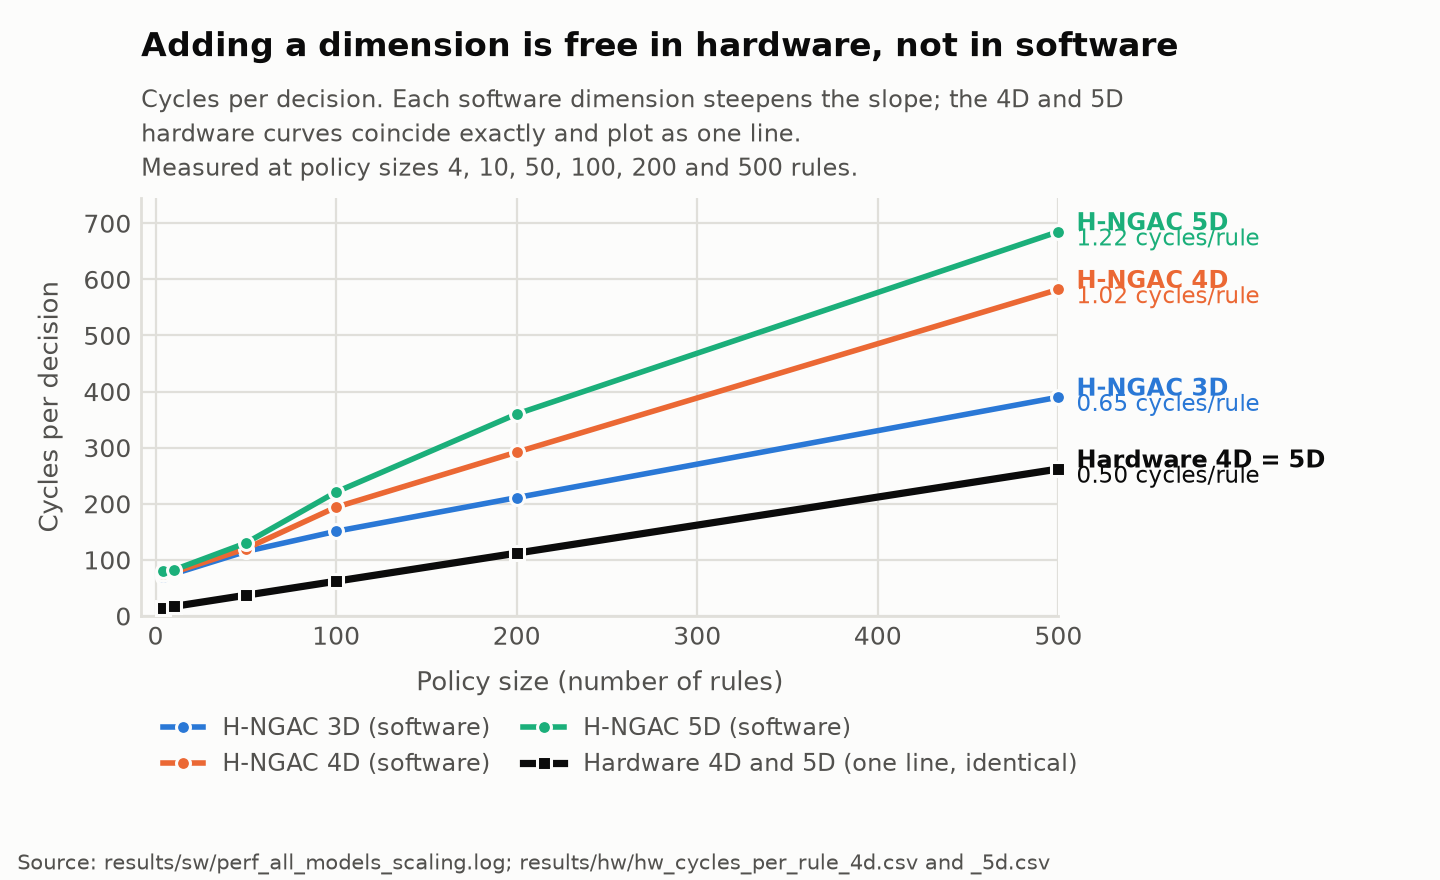
\includegraphics[width=\columnwidth]{chart-key-finding.png}
\caption{Cycles per decision versus policy size. Software slopes steepen with each added dimension. The 4D and 5D hardware series are identical at every measured point.}
\label{fig:keyfinding}
\end{figure}

\subsection{Faster baselines are faster because they are wrong}

Table~\ref{tab:models} compares six software models on the same corpus. The RBAC hash map resolves in roughly 100 derived cycles at every policy size, and the flat cost is genuine. However, it admits 200{,}000 of 200{,}000 requests in the April corpus, including all 100{,}000 that violate state, and the DAG-NGAC and three-dimensional paths admit the same. A model that cannot see the state or provenance dimensions cannot deny on them. The only software models that decide correctly are the five-dimensional path and a flattened direct-lookup table that trades a 19.7$\times$ memory footprint for its speed. However, an RBAC deployment could encode state into its role set, a maintenance operator role distinct from a normal operator role. Sixteen state bits and three source types multiply that role count combinatorially, and the honest alternative, RBAC consulting an external state store, cost 20.6 times the four-dimensional path when we measured it against an in-process SQLite store. It might be tempting to read Table~\ref{tab:models} as an argument that cheap static authorization suffices. The correctness column is the answer: the fast rows are fast because they answer a smaller question than the one Layla's interlock asks.

\begin{table}[t]
\caption{Software models, derived cycles per decision at 500 rules, and corpus correctness. ``Over'' = admits state- or provenance-violating requests.}
\label{tab:models}
\centering
\begin{tabular}{lrl}
\toprule
Model & Cycles (500) & Decides correctly? \\
\midrule
H-NGAC 3D & 390 & No, over-authorizes \\
H-NGAC 4D & 582 & No, over-authorizes \\
H-NGAC 5D & 685 & \textbf{Yes} \\
RBAC hash map & 100 & No, over-authorizes \\
DAG-NGAC traversal & 1{,}032 & No, over-authorizes \\
Flattened 5D lookup & 984 & \textbf{Yes}, 19.7$\times$ memory \\
\bottomrule
\end{tabular}
\end{table}

\subsection{Adversarial evaluation in ROS 2}

We ran the provenance-abuse scenario live. A software gatekeeper node executing the same five-dimensional decision function fronted an actuator topic while a legitimate node and a compromised node both published with valid credentials for the same authorized subject, the compromised node at five times the legitimate rate. Over a 30-second session the policy blocked 18{,}878 of 18{,}878 injection attempts, a block rate of 100\% with a one-sided 95\% Wilson lower bound of 99.99\%, and passed 17{,}059 of 17{,}059 legitimate commands, a false positive rate of 0\% with a 95\% upper bound of 0.02\%. This demo and the board run carry two separate claims. The demo establishes what the five-dimensional policy semantics block under sustained adversarial load. The silicon run establishes that the synthesized kernel computes identical decisions on all 2{,}307 corpus requests. Neither claim substitutes for the other. Under three- or four-dimensional policy every one of those injections would have been admitted, because the attacker's identity triple and state context were valid. Only the provenance dimension separates the two traffic streams.

The same runs measured the timing-window property. Under both idle and saturated CPU load, zero authorization callbacks of 8{,}733 exceeded the 50~$\mu$s lower bound of DDS localhost propagation. We report this strictly as a null result. The architectural argument stands on (4): a synthesis-time bound below the propagation floor closes the window by construction, which no measured software mean can do.

\subsection{The comparison we do not make, and the one we do}

It might be tempting to infer from Table~\ref{tab:cycles} that the fabric outpaces the CPU. That inference would be incorrect, and we pre-empt it. At 500 rules the i7 completes a mean five-dimensional decision in 138~ns of wall clock against the fabric's 2.62~$\mu$s, because a 4.96~GHz core is 49.6 times faster per cycle than a 100~MHz fabric. The CPU wins the mean by roughly 19$\times$. The defensible comparison is the worst case, and there the ordering reverses: the software path's worst observed decision at 200 rules was 355.4~$\mu$s against the fabric's invariant 1.12~$\mu$s, and its worst at four rules was 298.8~$\mu$s against 0.14~$\mu$s. Further, the software figure is an observation, not a bound. The 157~$\mu$s outlier in our DCAS baseline arrived in a run whose mean was 1.14~$\mu$s \cite{karim2026dcas}. An operating system does not guarantee its own tail, and a control loop budgets for the tail.

% AUTHOR DECISION: OPA/XACML reuse from TS-NGAC (approved for manuscript per
% canonical-context, flagged as open in manuscript-agent-prompt rule 8).
% Cut this paragraph if the journal contribution split argues otherwise.
For completeness we place general-purpose policy engines on the same axis. In our prior evaluation, Open Policy Agent averaged 271.491~$\mu$s per decision with 13 deadline misses \cite{karim2026tsngac}, and an XACML OpenPDP deployment averaged roughly 50~ms \cite{karim2026dcas, oasisxacml}. These engines evaluate far richer policy than (2) expresses, and we do not fault their generality. We observe only that they occupy a latency regime three to five orders of magnitude above the closed form of (4), which is the regime that keeps authorization out of control paths.

\section{Related Work}

We rate prior work on four axes, each an integer score $x \in \mathbb{Z},\ 0 \le x \le 5$: per-decision latency evidence ($\mathit{pdl}$), where 5 requires cycle-accurate per-decision measurement; worst-case boundedness ($\mathit{wcb}$), where 5 requires a closed-form bound verified at every measured point; enforcement dimensionality beyond the identity triple ($\mathit{dim}$), where 3 denotes one added runtime dimension and 5 denotes both state and provenance; and hardware validation ($\mathit{hwv}$), where 5 requires cycle-accurate co-simulation plus silicon functional verification. Table~\ref{tab:rubric} scores each line of prior work under these definitions. The paragraphs below justify the scores that matter most, and they concede three genuine ancestors plainly.

\begin{table}[t]
\caption{Related work scored on the four rubric axes.}
\label{tab:rubric}
\centering
\footnotesize
\setlength{\tabcolsep}{3.5pt}
\begin{tabular}{lcccc}
\toprule
Prior work & $\mathit{pdl}$ & $\mathit{wcb}$ & $\mathit{dim}$ & $\mathit{hwv}$ \\
\midrule
DAG-NGAC / Policy Machine \cite{incits565, ferraiolo2011policymachine} & 1 & 0 & 2 & 0 \\
Linear-time NGAC \cite{mell2017linear} & 3 & 1 & 2 & 0 \\
XEngine \cite{liu2011xengine} & 3 & 0 & 3 & 0 \\
OPA \cite{opa} & 3 & 0 & 3 & 0 \\
XACML PDP \cite{oasisxacml} & 2 & 0 & 3 & 0 \\
SROS2 / DDS-Security \cite{mayoralvilches2022sros2, omgddssec} & 2 & 0 & 0 & 0 \\
App-layer ROS authorization \cite{dieber2017security} & 2 & 0 & 1 & 0 \\
ROS-Defender \cite{rivera2019rosdefender} & 2 & 0 & 1 & 0 \\
ABAC for multi-robot systems \cite{salimi2025abac} & 2 & 0 & 3 & 0 \\
FPGA reference monitor \cite{huffmire2006policy} & 3 & 3 & 1 & 4 \\
NoC data protection units \cite{fiorin2008secure} & 3 & 3 & 1 & 3 \\
Bit-vector classification \cite{song2005bvtcam, ganegedara2014scalable} & 4 & 4 & 0 & 4 \\
SoC access-control wrappers \cite{restuccia2021aker} & 3 & 3 & 1 & 4 \\
CHERI \cite{watson2015cheri} & 4 & 4 & 0 & 5 \\
Security-aware RT scheduling \cite{hasan2017contego, lesi2017security, hasan2024sok} & 3 & 2 & 1 & 0 \\
CPS runtime enforcement \cite{pinisetty2017runtime} & 2 & 3 & 1 & 0 \\
HyperNGAC \cite{sitharaman2025hypergraph} & 0 & 0 & 3 & 0 \\
H-NGAC \cite{karim2026dcas} & 4 & 2 & 0 & 1 \\
TS-NGAC \cite{karim2026tsngac} & 4 & 3 & 3 & 0 \\
\textbf{This work} & \textbf{5} & \textbf{5} & \textbf{5} & \textbf{5} \\
\bottomrule
\end{tabular}
\end{table}

\textbf{Software policy engines and models.} The NGAC standard and the Policy Machine define the model we compile but report no per-decision latency evidence \cite{incits565, ferraiolo2011policymachine, hu2014sp800162}, and NGAC's decision and review advantages over XACML are established in the standards comparison of Ferraiolo et al.\ \cite{ferraiolo2016xacml}. NGAC implementations to date are software, including NIST's own fine-grain enforcement over database queries \cite{ferraiolo2017database}, and the strongest software NGAC decision result is the linear-time graph algorithms of Mell et al.\ \cite{mell2017linear}. That is the right software bound, and it is still a per-decision traversal whose constant depends on the host. XEngine compiles XACML into numeric structures offline and speeds decisions by orders of magnitude \cite{liu2011xengine}, the closest software analogue of our compilation step, but its decision latency still varies with policy and request shape. Servos and Osborn's survey lists ABAC decision performance among the field's open problems \cite{servos2017abac}, and our own measurements place OPA and an XACML PDP three to five orders of magnitude above (4) \cite{opa, karim2026tsngac, oasisxacml}.

\textbf{Hardware enforcement.} This literature holds three genuine ancestors, and we cite them as such. Huffmire et al.\ compiled a formally specified memory-isolation policy directly into an FPGA reference monitor in 2006 \cite{huffmire2006policy}, and Fiorin et al.\ placed access-rights checks into NoC interfaces with no added latency on the authorized path \cite{fiorin2008secure}. Both make enforcement latency a property of a synthesized circuit. Neither evaluates a relational policy model, and neither analyzes what an added policy dimension costs. The third concession is packet classification: TCAM and bit-vector engines match wide multi-field keys at deterministic rates \cite{song2005bvtcam}, and the StrideBV line advertises latency independent of ruleset content \cite{ganegedara2014scalable}. However, StrideBV latency grows linearly with match-key width. That is, in the closest deterministic prior art, added dimensions are precisely not free in time, which is the axis this paper claims. Aker wraps SoC controllers in verified access-control hardware at the bus-transaction level \cite{restuccia2021aker}, and CHERI enforces per-instruction memory capabilities in silicon \cite{watson2015cheri}. Both police a lower layer than a policy model.

\textbf{Real-time and robot security.} The real-time security literature schedules software enforcement around deadlines: Contego slots security tasks into scheduling slack \cite{hasan2017contego}, Lesi et al.\ trade control quality against integrity checking \cite{lesi2017security}, and the 2024 SoK catalogs the paradigm \cite{hasan2024sok}. We exit that paradigm rather than optimize within it, since a fabric decision consumes no CPU slack at all. Pinisetty et al.\ synthesize runtime enforcers from timed automata for reactive CPS \cite{pinisetty2017runtime}, the nearest formal-synthesis neighbor, targeting safety properties rather than authorization and offering no hardware latency model. In robotics, Dieber et al.\ argued for application-layer authorization above transport crypto with identity-based decisions \cite{dieber2017security}, ROS-Defender filters node flows at the network layer \cite{rivera2019rosdefender}, and Salimi et al.\ condition per-request ABAC decisions on task and capability attributes through a blockchain bridge \cite{salimi2025abac}. None conditions a command on its source type or the platform's runtime safety state, and none is an inline bounded-latency primitive.

Since this work measures cycle-accurate per-decision latency, verifies a closed-form bound at every measured point, enforces both state and provenance, and validates through co-simulation and silicon functional verification, we assign it the maximum on all four axes under the definitions above. We state the novelty claim in its bounded form. Constant-latency wide-key matching exists in TCAMs, deterministic classification exists in the bit-vector family, and policy-to-circuit compilation dates to 2006. To our knowledge, no prior work compiles a standardized relational authorization model to hardware and demonstrates, on identical toolflow and part, that added policy dimensions cost zero clock cycles, and no prior hardware implementation of NGAC exists at all. We invite correction on both points.

\section{Limitations}

Our claims are bounded by several factors, and we state them plainly. First, the three-dimensional kernel was never synthesized and its kernel code no longer exists, thus every hardware parity claim in this paper is scoped to four versus five dimensions. Second, no on-board timing exists. Cycle counts come from cycle-accurate co-simulation, and the silicon run verifies function only. Third, the software baseline is a 4.96~GHz laptop CPU while the fabric runs at 100~MHz; an embedded-class CPU baseline on the board's own Cortex-A9 would make the wall-clock comparison fairer to the fabric, and we did not run it. Fourth, software latency distributions were measured under WSL2, whose scheduler jitter contaminates maxima, which is why we cite worst observed values and never call them WCETs. Fifth, the primitive is capacity-bounded at 512 rules and 256 policy nodes, and policy update happens off the decision path. Sixth, one baseline, the modeled external-state lookup, is synthetic, and we excluded it from every empirical claim after finding it added nothing the measured SQLite path does not show. Seventh, the kernel compiles only the association subset of INCITS 565. Prohibitions, obligations and administrative relations are not implemented, so no claim here extends beyond rules that grant. Eighth, the zero-cycle result is demonstrated at one operating point, 100~MHz on a Zynq-7020, where both kernels close timing with identical +0.33~ns slack. At an aggressive clock target the added dimension could force an additional pipeline stage, which is exactly the boundary the hypothesis of Section~III predicts. Characterizing that frequency ceiling is future work.

\section{Future Work and Conclusion}

Four questions structure our next steps. 1.~Can a re-derived three-dimensional kernel restore the full three-way parity claim in synthesis? 2.~What measurement path yields trustworthy on-board cycle counts on Zynq-class parts? 3.~Does the closed form of (4) survive a dynamic policy update path, or does update traffic reintroduce jitter? 4.~How does the primitive compose with time-scoped delegation, which our journal-track work develops in software? Further, we call on the community to report authorization performance as cycle-level worst cases rather than means, because a mean is precisely the statistic a control loop cannot budget against.

In conclusion, we extended the H-NGAC bitmask primitive with system-state and command-provenance dimensions and synthesized both the four- and five-dimensional kernels to a Zynq-7020. The added dimension costs zero clock cycles and 524 LUTs, latency is closed-form at $12 + n/2$ cycles with zero jitter by construction, and the five-dimensional policy blocked 18{,}878 of 18{,}878 credentialed injection attempts in ROS~2 with zero false positives in 17{,}059 legitimate commands. Robotics platform engineers and functional-safety engineers can treat the authorization worst case as a synthesis parameter, place the decision inside the control loop budget, and close the two attack classes that identity-based authorization admits. Layla's interlock becomes a policy bit the fabric checks in bounded time, not a procedure she hopes the operator follows.

\bibliographystyle{IEEEtran}
\bibliography{refs}

\end{document}
